\documentclass{ximera}

%\usepackage{todonotes}

\newcommand{\todo}{}

\usepackage{esint} % for \oiint
\ifxake%%https://math.meta.stackexchange.com/questions/9973/how-do-you-render-a-closed-surface-double-integral
\renewcommand{\oiint}{{\large\bigcirc}\kern-1.56em\iint}
\fi


\graphicspath{
  {./}
  {ximeraTutorial/}
  {basicPhilosophy/}
  {functionsOfSeveralVariables/}
  {normalVectors/}
  {lagrangeMultipliers/}
  {vectorFields/}
  {greensTheorem/}
  {shapeOfThingsToCome/}
  {dotProducts/}
  {partialDerivativesAndTheGradientVector/}
  {../productAndQuotientRules/exercises/}
  {../normalVectors/exercisesParametricPlots/}
  {../continuityOfFunctionsOfSeveralVariables/exercises/}
  {../partialDerivativesAndTheGradientVector/exercises/}
  {../directionalDerivativeAndChainRule/exercises/}
  {../commonCoordinates/exercisesCylindricalCoordinates/}
  {../commonCoordinates/exercisesSphericalCoordinates/}
  {../greensTheorem/exercisesCurlAndLineIntegrals/}
  {../greensTheorem/exercisesDivergenceAndLineIntegrals/}
  {../shapeOfThingsToCome/exercisesDivergenceTheorem/}
  {../greensTheorem/}
  {../shapeOfThingsToCome/}
  {../separableDifferentialEquations/exercises/}
  {vectorFields/}
}

\newcommand{\mooculus}{\textsf{\textbf{MOOC}\textnormal{\textsf{ULUS}}}}

\usepackage{tkz-euclide}
\usepackage{tikz}
\usepackage{tikz-cd}
\usetikzlibrary{arrows}
\tikzset{>=stealth,commutative diagrams/.cd,
  arrow style=tikz,diagrams={>=stealth}} %% cool arrow head
\tikzset{shorten <>/.style={ shorten >=#1, shorten <=#1 } } %% allows shorter vectors

\usetikzlibrary{backgrounds} %% for boxes around graphs
\usetikzlibrary{shapes,positioning}  %% Clouds and stars
\usetikzlibrary{matrix} %% for matrix
\usepgfplotslibrary{polar} %% for polar plots
\usepgfplotslibrary{fillbetween} %% to shade area between curves in TikZ
%\usetkzobj{all}
\usepackage[makeroom]{cancel} %% for strike outs
%\usepackage{mathtools} %% for pretty underbrace % Breaks Ximera
%\usepackage{multicol}
\usepackage{pgffor} %% required for integral for loops



%% http://tex.stackexchange.com/questions/66490/drawing-a-tikz-arc-specifying-the-center
%% Draws beach ball
\tikzset{pics/carc/.style args={#1:#2:#3}{code={\draw[pic actions] (#1:#3) arc(#1:#2:#3);}}}



\usepackage{array}
\setlength{\extrarowheight}{+.1cm}
\newdimen\digitwidth
\settowidth\digitwidth{9}
\def\divrule#1#2{
\noalign{\moveright#1\digitwidth
\vbox{\hrule width#2\digitwidth}}}




% \newcommand{\RR}{\mathbb R}
% \newcommand{\R}{\mathbb R}
% \newcommand{\N}{\mathbb N}
% \newcommand{\Z}{\mathbb Z}

\newcommand{\sagemath}{\textsf{SageMath}}


%\renewcommand{\d}{\,d\!}
%\renewcommand{\d}{\mathop{}\!d}
%\newcommand{\dd}[2][]{\frac{\d #1}{\d #2}}
%\newcommand{\pp}[2][]{\frac{\partial #1}{\partial #2}}
% \renewcommand{\l}{\ell}
%\newcommand{\ddx}{\frac{d}{\d x}}

% \newcommand{\zeroOverZero}{\ensuremath{\boldsymbol{\tfrac{0}{0}}}}
%\newcommand{\inftyOverInfty}{\ensuremath{\boldsymbol{\tfrac{\infty}{\infty}}}}
%\newcommand{\zeroOverInfty}{\ensuremath{\boldsymbol{\tfrac{0}{\infty}}}}
%\newcommand{\zeroTimesInfty}{\ensuremath{\small\boldsymbol{0\cdot \infty}}}
%\newcommand{\inftyMinusInfty}{\ensuremath{\small\boldsymbol{\infty - \infty}}}
%\newcommand{\oneToInfty}{\ensuremath{\boldsymbol{1^\infty}}}
%\newcommand{\zeroToZero}{\ensuremath{\boldsymbol{0^0}}}
%\newcommand{\inftyToZero}{\ensuremath{\boldsymbol{\infty^0}}}



% \newcommand{\numOverZero}{\ensuremath{\boldsymbol{\tfrac{\#}{0}}}}
% \newcommand{\dfn}{\textbf}
% \newcommand{\unit}{\,\mathrm}
% \newcommand{\unit}{\mathop{}\!\mathrm}
% \newcommand{\eval}[1]{\bigg[ #1 \bigg]}
% \newcommand{\seq}[1]{\left( #1 \right)}
% \renewcommand{\epsilon}{\varepsilon}
% \renewcommand{\phi}{\varphi}


% \renewcommand{\iff}{\Leftrightarrow}

% \DeclareMathOperator{\arccot}{arccot}
% \DeclareMathOperator{\arcsec}{arcsec}
% \DeclareMathOperator{\arccsc}{arccsc}
% \DeclareMathOperator{\si}{Si}
% \DeclareMathOperator{\scal}{scal}
% \DeclareMathOperator{\sign}{sign}


%% \newcommand{\tightoverset}[2]{% for arrow vec
%%   \mathop{#2}\limits^{\vbox to -.5ex{\kern-0.75ex\hbox{$#1$}\vss}}}
% \newcommand{\arrowvec}[1]{{\overset{\rightharpoonup}{#1}}}
% \renewcommand{\vec}[1]{\arrowvec{\mathbf{#1}}}
% \renewcommand{\vec}[1]{{\overset{\boldsymbol{\rightharpoonup}}{\mathbf{#1}}}}

% \newcommand{\point}[1]{\left(#1\right)} %this allows \vector{ to be changed to \vector{ with a quick find and replace
% \newcommand{\pt}[1]{\mathbf{#1}} %this allows \vec{ to be changed to \vec{ with a quick find and replace
% \newcommand{\Lim}[2]{\lim_{\point{#1} \to \point{#2}}} %Bart, I changed this to point since I want to use it.  It runs through both of the exercise and exerciseE files in limits section, which is why it was in each document to start with.

% \DeclareMathOperator{\proj}{\mathbf{proj}}
% \newcommand{\veci}{{\boldsymbol{\hat{\imath}}}}
% \newcommand{\vecj}{{\boldsymbol{\hat{\jmath}}}}
% \newcommand{\veck}{{\boldsymbol{\hat{k}}}}
% \newcommand{\vecl}{\vec{\boldsymbol{\l}}}
% \newcommand{\uvec}[1]{\mathbf{\hat{#1}}}
% \newcommand{\utan}{\mathbf{\hat{t}}}
% \newcommand{\unormal}{\mathbf{\hat{n}}}
% \newcommand{\ubinormal}{\mathbf{\hat{b}}}

% \newcommand{\dotp}{\bullet}
% \newcommand{\cross}{\boldsymbol\times}
% \newcommand{\grad}{\boldsymbol\nabla}
% \newcommand{\divergence}{\grad\dotp}
% \newcommand{\curl}{\grad\cross}
%\DeclareMathOperator{\divergence}{divergence}
%\DeclareMathOperator{\curl}[1]{\grad\cross #1}
% \newcommand{\lto}{\mathop{\longrightarrow\,}\limits}

% \renewcommand{\bar}{\overline}

\colorlet{textColor}{black}
\colorlet{background}{white}
\colorlet{penColor}{blue!50!black} % Color of a curve in a plot
\colorlet{penColor2}{red!50!black}% Color of a curve in a plot
\colorlet{penColor3}{red!50!blue} % Color of a curve in a plot
\colorlet{penColor4}{green!50!black} % Color of a curve in a plot
\colorlet{penColor5}{orange!80!black} % Color of a curve in a plot
\colorlet{penColor6}{yellow!70!black} % Color of a curve in a plot
\colorlet{fill1}{penColor!20} % Color of fill in a plot
\colorlet{fill2}{penColor2!20} % Color of fill in a plot
\colorlet{fillp}{fill1} % Color of positive area
\colorlet{filln}{penColor2!20} % Color of negative area
\colorlet{fill3}{penColor3!20} % Fill
\colorlet{fill4}{penColor4!20} % Fill
\colorlet{fill5}{penColor5!20} % Fill
\colorlet{gridColor}{gray!50} % Color of grid in a plot

\newcommand{\surfaceColor}{violet}
\newcommand{\surfaceColorTwo}{redyellow}
\newcommand{\sliceColor}{greenyellow}




\pgfmathdeclarefunction{gauss}{2}{% gives gaussian
  \pgfmathparse{1/(#2*sqrt(2*pi))*exp(-((x-#1)^2)/(2*#2^2))}%
}


%%%%%%%%%%%%%
%% Vectors
%%%%%%%%%%%%%

%% Simple horiz vectors
\renewcommand{\vector}[1]{\left\langle #1\right\rangle}


%% %% Complex Horiz Vectors with angle brackets
%% \makeatletter
%% \renewcommand{\vector}[2][ , ]{\left\langle%
%%   \def\nextitem{\def\nextitem{#1}}%
%%   \@for \el:=#2\do{\nextitem\el}\right\rangle%
%% }
%% \makeatother

%% %% Vertical Vectors
%% \def\vector#1{\begin{bmatrix}\vecListA#1,,\end{bmatrix}}
%% \def\vecListA#1,{\if,#1,\else #1\cr \expandafter \vecListA \fi}

%%%%%%%%%%%%%
%% End of vectors
%%%%%%%%%%%%%

%\newcommand{\fullwidth}{}
%\newcommand{\normalwidth}{}



%% makes a snazzy t-chart for evaluating functions
%\newenvironment{tchart}{\rowcolors{2}{}{background!90!textColor}\array}{\endarray}

%%This is to help with formatting on future title pages.
\newenvironment{sectionOutcomes}{}{}



%% Flowchart stuff
%\tikzstyle{startstop} = [rectangle, rounded corners, minimum width=3cm, minimum height=1cm,text centered, draw=black]
%\tikzstyle{question} = [rectangle, minimum width=3cm, minimum height=1cm, text centered, draw=black]
%\tikzstyle{decision} = [trapezium, trapezium left angle=70, trapezium right angle=110, minimum width=3cm, minimum height=1cm, text centered, draw=black]
%\tikzstyle{question} = [rectangle, rounded corners, minimum width=3cm, minimum height=1cm,text centered, draw=black]
%\tikzstyle{process} = [rectangle, minimum width=3cm, minimum height=1cm, text centered, draw=black]
%\tikzstyle{decision} = [trapezium, trapezium left angle=70, trapezium right angle=110, minimum width=3cm, minimum height=1cm, text centered, draw=black]


\title{Piecewise Intersection}

\begin{document}

\begin{abstract}
equations
\end{abstract}
\maketitle





Below are two piecewise defined functions and their graphs: $V(h)$ and $K(m)$. 







\[
V(h) = 
\begin{cases}
  -2h-3 & \text{ if } [-6, -2]   \\
  -(h+3)(h-3) & \text{ if } (-2, 4]  \\
  \frac{7h}{4} - 8 & \text{ if } (4,8)
\end{cases}
\]







\begin{image}
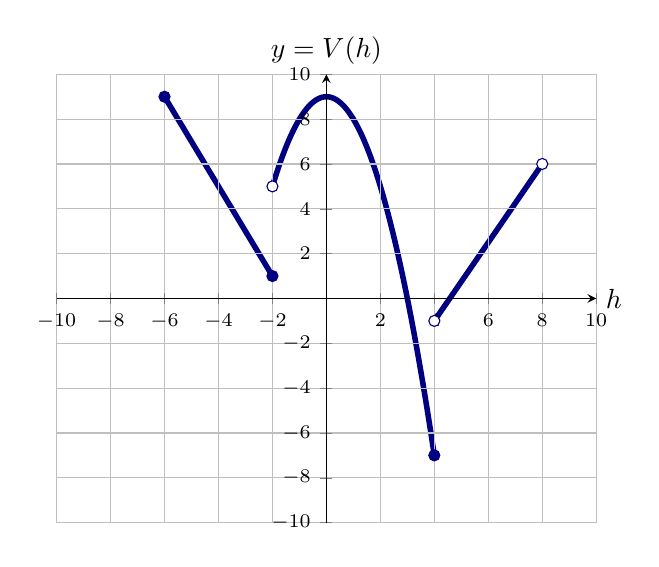
\begin{tikzpicture}
  \begin{axis}[
            domain=-10:10, ymax=10, xmax=10, ymin=-10, xmin=-10,
            axis lines =center, xlabel=$h$, ylabel={$y=V(h)$}, grid = major,
            ytick={-10,-8,-6,-4,-2,2,4,6,8,10},
            xtick={-10,-8,-6,-4,-2,2,4,6,8,10},
            ticklabel style={font=\scriptsize},
            every axis y label/.style={at=(current axis.above origin),anchor=south},
            every axis x label/.style={at=(current axis.right of origin),anchor=west},
            axis on top
          ]
          
			\addplot [line width=2, penColor, smooth,samples=100,domain=(-6:-2)] {-2*x-3};
       		\addplot [line width=2, penColor, smooth,samples=100,domain=(-2:4)] {-1*(x+3)*(x-3))};
       		\addplot [line width=2, penColor, smooth,samples=100,domain=(4:8)] {1.75*x-8};




			\addplot[color=penColor,fill=penColor,only marks,mark=*] coordinates{(-6,9)};
			\addplot[color=penColor,fill=penColor,only marks,mark=*] coordinates{(-2,1)};

			\addplot[color=penColor,fill=white,only marks,mark=*] coordinates{(-2,5)};
			\addplot[color=penColor,fill=penColor,only marks,mark=*] coordinates{(4,-7)};

			\addplot[color=penColor,fill=white,only marks,mark=*] coordinates{(4,-1)};
			\addplot[color=penColor,fill=white,only marks,mark=*] coordinates{(8,6)};


           

  \end{axis}
\end{tikzpicture}
\end{image}




\[
K(m) = 
\begin{cases}
  m+4 & \text{ if } (-7, 0]   \\
  m^2-7m+9 & \text{ if } (1,6]
\end{cases}
\]



\begin{image}
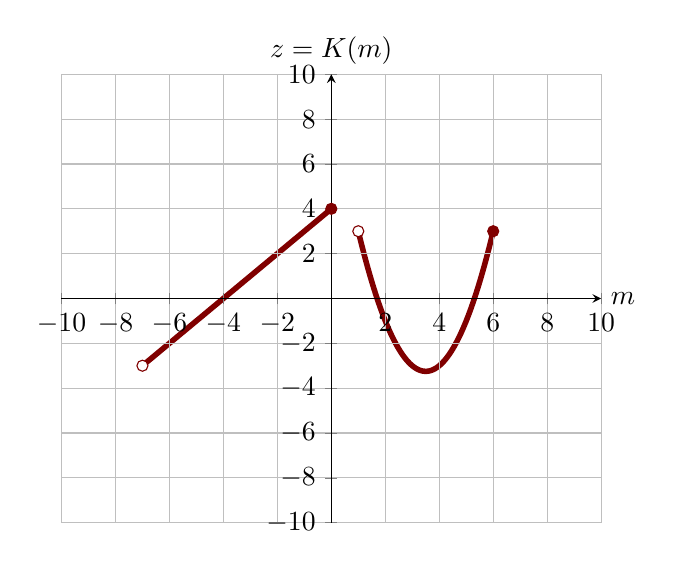
\begin{tikzpicture} 
  \begin{axis}[
            domain=-10:10, ymax=10, xmax=10, ymin=-10, xmin=-10,
            axis lines =center, xlabel=$m$, ylabel={$z=K(m)$}, grid = major,
            ytick={-10,-8,-6,-4,-2,2,4,6,8,10},
        	xtick={-10,-8,-6,-4,-2,2,4,6,8,10},
            every axis y label/.style={at=(current axis.above origin),anchor=south},
            every axis x label/.style={at=(current axis.right of origin),anchor=west},
            axis on top
          ]
          
			\addplot [line width=2, penColor2, smooth,samples=100,domain=(-7:0)] {x+4};
       		\addplot [line width=2, penColor2, smooth,samples=100,domain=(1:6)] {(x-1)*(x-6)+3};



			\addplot[color=penColor2,fill=white,only marks,mark=*] coordinates{(-7,-3)};
			\addplot[color=penColor2,fill=penColor2,only marks,mark=*] coordinates{(0,4)};

			\addplot[color=penColor2,fill=white,only marks,mark=*] coordinates{(1,3)};
			\addplot[color=penColor2,fill=penColor2,only marks,mark=*] coordinates{(6,3)};

       

  \end{axis}
\end{tikzpicture}
\end{image}



Find the points of intersection between the graphs of $V$ and $K$.


From the graphs there appear to be three points of intersection.

\section{First Point}




\begin{image}
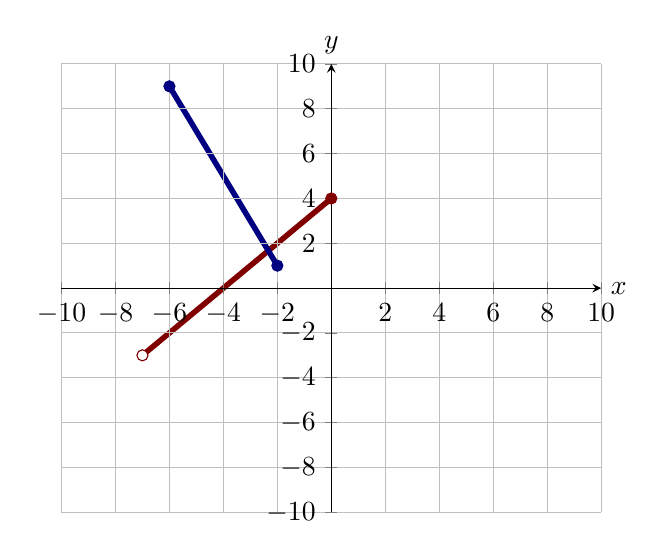
\begin{tikzpicture} 
  \begin{axis}[
            domain=-10:10, ymax=10, xmax=10, ymin=-10, xmin=-10,
            axis lines =center, xlabel=$x$, ylabel=$y$, grid = major,
            ytick={-10,-8,-6,-4,-2,2,4,6,8,10},
        	xtick={-10,-8,-6,-4,-2,2,4,6,8,10},
            every axis y label/.style={at=(current axis.above origin),anchor=south},
            every axis x label/.style={at=(current axis.right of origin),anchor=west},
            axis on top
          ]
          
			\addplot [line width=2, penColor2, smooth,samples=100,domain=(-7:0)] {x+4};
       		\addplot [line width=2, penColor, smooth,samples=100,domain=(-6:-2)] {-2*x-3};



			\addplot[color=penColor2,fill=white,only marks,mark=*] coordinates{(-7,-3)};
			\addplot[color=penColor2,fill=penColor2,only marks,mark=*] coordinates{(0,4)};
			\addplot[color=penColor,fill=penColor,only marks,mark=*] coordinates{(-6,9)};
			\addplot[color=penColor,fill=penColor,only marks,mark=*] coordinates{(-2,1)};

       

  \end{axis}
\end{tikzpicture}
\end{image}


\begin{question}


We'll set the function formulas equal to each other and solve the equation formed.



\[ -2x-3 =   \answer{x+4}       \]


\[ \answer{-3x} =  7      \]

\[ x =  \frac{7}{-3}   =  -\frac{7}{3}      \]
\end{question}





Check....
\begin{itemize}
\item $V(-\tfrac{7}{3}) = -2 \cdot -\tfrac{7}{3} - 3 = \tfrac{14}{3} - \tfrac{9}{3} = \tfrac{5}{3}$
\item $K(-\tfrac{7}{3}) =   -\tfrac{7}{3} + 4 =  -\tfrac{7}{3} + \frac{12}{3} = \tfrac{5}{3} $
\end{itemize}


The intersection point is $\left( -\frac{7}{3}, \frac{5}{3} \right)$.








\section{Second Point}




\begin{image}
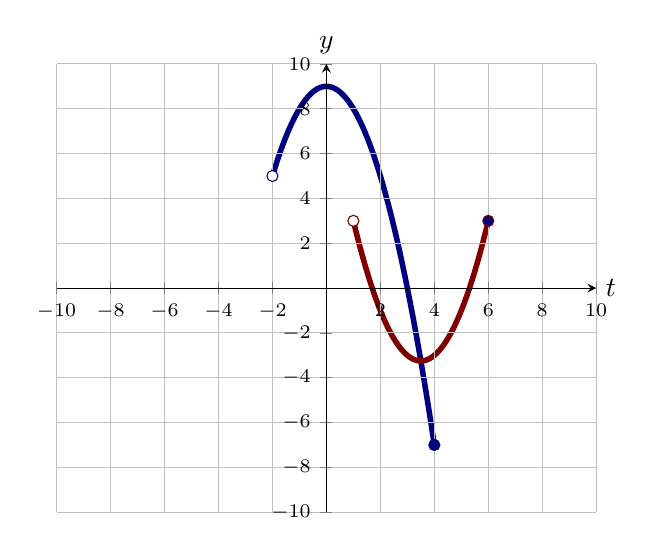
\begin{tikzpicture}
  \begin{axis}[
            domain=-10:10, ymax=10, xmax=10, ymin=-10, xmin=-10,
            axis lines =center, xlabel=$t$, ylabel=$y$, grid = major,
            ytick={-10,-8,-6,-4,-2,2,4,6,8,10},
            xtick={-10,-8,-6,-4,-2,2,4,6,8,10},
            ticklabel style={font=\scriptsize},
            every axis y label/.style={at=(current axis.above origin),anchor=south},
            every axis x label/.style={at=(current axis.right of origin),anchor=west},
            axis on top
          ]
          

       		\addplot [line width=2, penColor, smooth,samples=100,domain=(-2:4)] {-1*(x+3)*(x-3))};
			\addplot [line width=2, penColor2, smooth,samples=100,domain=(1:6)] {(x-1)*(x-6)+3};



			\addplot[color=penColor2,fill=white,only marks,mark=*] coordinates{(1,3)};
			\addplot[color=penColor2,fill=penColor,only marks,mark=*] coordinates{(6,3)};

			\addplot[color=penColor,fill=white,only marks,mark=*] coordinates{(-2,5)};
			\addplot[color=penColor,fill=penColor,only marks,mark=*] coordinates{(4,-7)};

		

           

  \end{axis}
\end{tikzpicture}
\end{image}




\begin{question}


We'll set the function formulas equal to each other and solve the equation formed.


\begin{align*}
\answer{-(t+3)(t-3)} &= t^2 - 7 t + 9  \\
\answer{-t^2 + 9}    &= t^2 - 7 t + 9 \\
0           &= 2 t^2 - 7t \\
0           &= t(2t - 7)  
\end{align*}
\end{question}





This gives two solutions, $0$ and $\frac{7}{2}$.  


We can see from the graph that the full graphs of $-(t+3)(t-3)$ and $t^2 - 7 t + 9$ would intersect at $t = 0$ as well.  However, our piecewise defined functions do not share these formulas at $0$.  The definitions of the piecewise functions do not allow $0$ as a common solution.

After considering the domains of $V$ and $H$, the only solution here is $\frac{7}{2}$.






Check....
\begin{itemize}
\item $V(\tfrac{7}{2}) = -\left(\tfrac{7}{2} + 3\right) \left(\tfrac{7}{2} - 3\right) = -\tfrac{13}{2}  \cdot \tfrac{1}{2} = -\frac{13}{4}$
\item $K(\tfrac{7}{2}) =   \left(\tfrac{7}{2}\right)^2 - 7\left(\tfrac{7}{2}\right) + 9 = -\frac{13}{4}$
\end{itemize}


The intersection point is $\left(\tfrac{7}{2}, -\frac{13}{4}\right)$.

















\section{Third Point}




\begin{image}
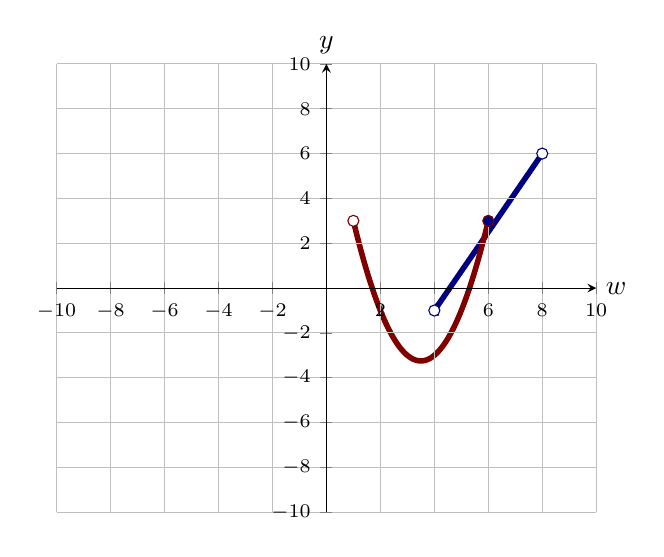
\begin{tikzpicture}
  \begin{axis}[
            domain=-10:10, ymax=10, xmax=10, ymin=-10, xmin=-10,
            axis lines =center, xlabel=$w$, ylabel=$y$, grid = major,
            ytick={-10,-8,-6,-4,-2,2,4,6,8,10},
            xtick={-10,-8,-6,-4,-2,2,4,6,8,10},
            ticklabel style={font=\scriptsize},
            every axis y label/.style={at=(current axis.above origin),anchor=south},
            every axis x label/.style={at=(current axis.right of origin),anchor=west},
            axis on top
          ]
          

       		\addplot [line width=2, penColor, smooth,samples=100,domain=(4:8)] {1.75*x-8};


			\addplot[color=penColor,fill=white,only marks,mark=*] coordinates{(4,-1)};
			\addplot[color=penColor,fill=white,only marks,mark=*] coordinates{(8,6)};

			\addplot [line width=2, penColor2, smooth,samples=100,domain=(1:6)] {(x-1)*(x-6)+3};



			\addplot[color=penColor2,fill=white,only marks,mark=*] coordinates{(1,3)};
			\addplot[color=penColor2,fill=penColor,only marks,mark=*] coordinates{(6,3)};

           

  \end{axis}
\end{tikzpicture}
\end{image}





\begin{question}


We'll set the function formulas equal to each other and solve the equation formed.

\begin{align*}
\answer{\frac{7w}{4} - 8}    &= w^2 - 7 w + 9     \\
0               &= w^2 - \answer{\frac{35w}{4}} + 17  \\
0           &= \frac{-(- \tfrac{35}{4}) \pm  \sqrt{(- \tfrac{35}{4})^2 - 4 \cdot 1 \cdot 17}}{2 \cdot 1} t \\
0           &= \frac{\tfrac{35}{4} \pm  \sqrt{\tfrac{137}{16}}}{2}  \\
0           &=   \frac{35}{8} \pm  \frac{\sqrt{137}}{8} \\
0          &= \frac{35 \pm \sqrt{137}}{8} 
\end{align*}

\end{question}





The graph shows us that we only have one of these solutions because the line segment doesn't extend further to the left to intersect the parabola twice.


The only soution here is $w = \frac{35 + \sqrt{137}}{8} $.








Check....
\begin{itemize}
\item $V\left(\frac{35 + \sqrt{137}}{8}\right) =  \frac{1}{32}(7 \sqrt{137} - 11)  $




\item $K\left(\frac{35 + \sqrt{137}}{8}\right) =  \frac{1}{32}(7 \sqrt{137} - 11)  $
\end{itemize}

\begin{question}
The intersection point is $\left(\frac{35 + \sqrt{137}}{8}, \answer{\frac{1}{32}(7 \sqrt{137} - 11)} \right)$.
\end{question}
















\begin{center}
\textbf{\textcolor{green!50!black}{ooooo-=-=-=-ooOoo-=-=-=-ooooo}} \\

more examples can be found by following this link\\ \link[More Examples of Piecewise-Defined Functions]{https://ximera.osu.edu/csccmathematics/precalculus1/precalculus1/piecewiseAnalysis/examples/exampleList}

\end{center}








\end{document}
